\section{Systematic uncertainties}
\label{sec:syst}

\todo{fix citations}
\subsection{Theory uncertainties}
\label{ssec:theoryuncert}
The estimation of the CP BSM parameters\todo{mention explicitly} from the OO shape requires the precise knowledge of the SM contributions and related uncertainties. This includes both SM gluon-gluon fusion (background) and SM VBF (signal).
 Therefore, the different theoretical uncertainties affecting the SM predictions are included in the fitting likelihood. This includes uncertainties from PDF, QCD order and $\alpha_s$.

For the gluon-fusion production mode, nine uncertainty sources are used to model the QCD theory
uncertainties, following the recommendation of the LHC Higgs cross section working group~\cite{LHCXS_4}. These sources are:
\begin{itemize}
\item two sources correspond to yield uncertainties related to the total cross section. Their magnitude is taken from the
STWZ-BLPTW predictions~\cite{ggF_qcd_unc_1,ggF_qcd_unc_2,LHCXS_4} and their impact on the different bins is evaluated using
NNLOPS.
\item two sources correspond to migration uncertainties related to splitting the phase space by jet multiplicity. Their magnitude and impact are derived similarly to the yield uncertainties
\item two uncertainty sources are related to the $p_\mathrm{T}^H$ shape and are estimated from scale
variations in NNLOPS, including variations of the HNNLO input scales and the renormalization
and factorization scales in Powheg.
\item two uncertainty sources related to the enhancement of uncertainties for events with typical VBF topology (due to explicit or implicit third-jet vetos), and are estimated by scale variations in MCFM~\cite{MCFM}, and the corresponding uncertainties are estimated using the same procedure use for yield and migration uncertainties.
\item one uncertainty source is related to the treatment of $m_t$ and is most important at large $p_\mathrm{T}^H$.
\end{itemize}

Following the recommendations of PDF4LHC~\cite{pdf4lhc}, the PDF uncertainties are evaluated using the 30 eigenvectors\todo{eigenvariations} set and treating each of them as an uncorrelated source. One additional nuisance parameter accounts for the uncertainties in $\alpha_{s}$.

For the $VBF+VH$ production modes, QCD uncertainties are estimated as an envelope of the scale variations available in Powheg~\cite{Nason:2009ai,VBFVH_theoryUnc}. Uncertainties from the choice of the PDF set and $\alpha_\mathrm{s}$ are evaluated similar to the gluon-fusion case.
A summary of the magnitude of these uncertainties in the different categories and OO bins is shown in the Figure ~\ref{fig:theoryUnc_ggF} ~\ref{fig:theoryUnc_VBF}.
\todo{add a comment on the rough size of these uncertainties}
\todo{plots are too small}
\begin{figure}[htbp]
\centering
  \subfloat[TT ]{ 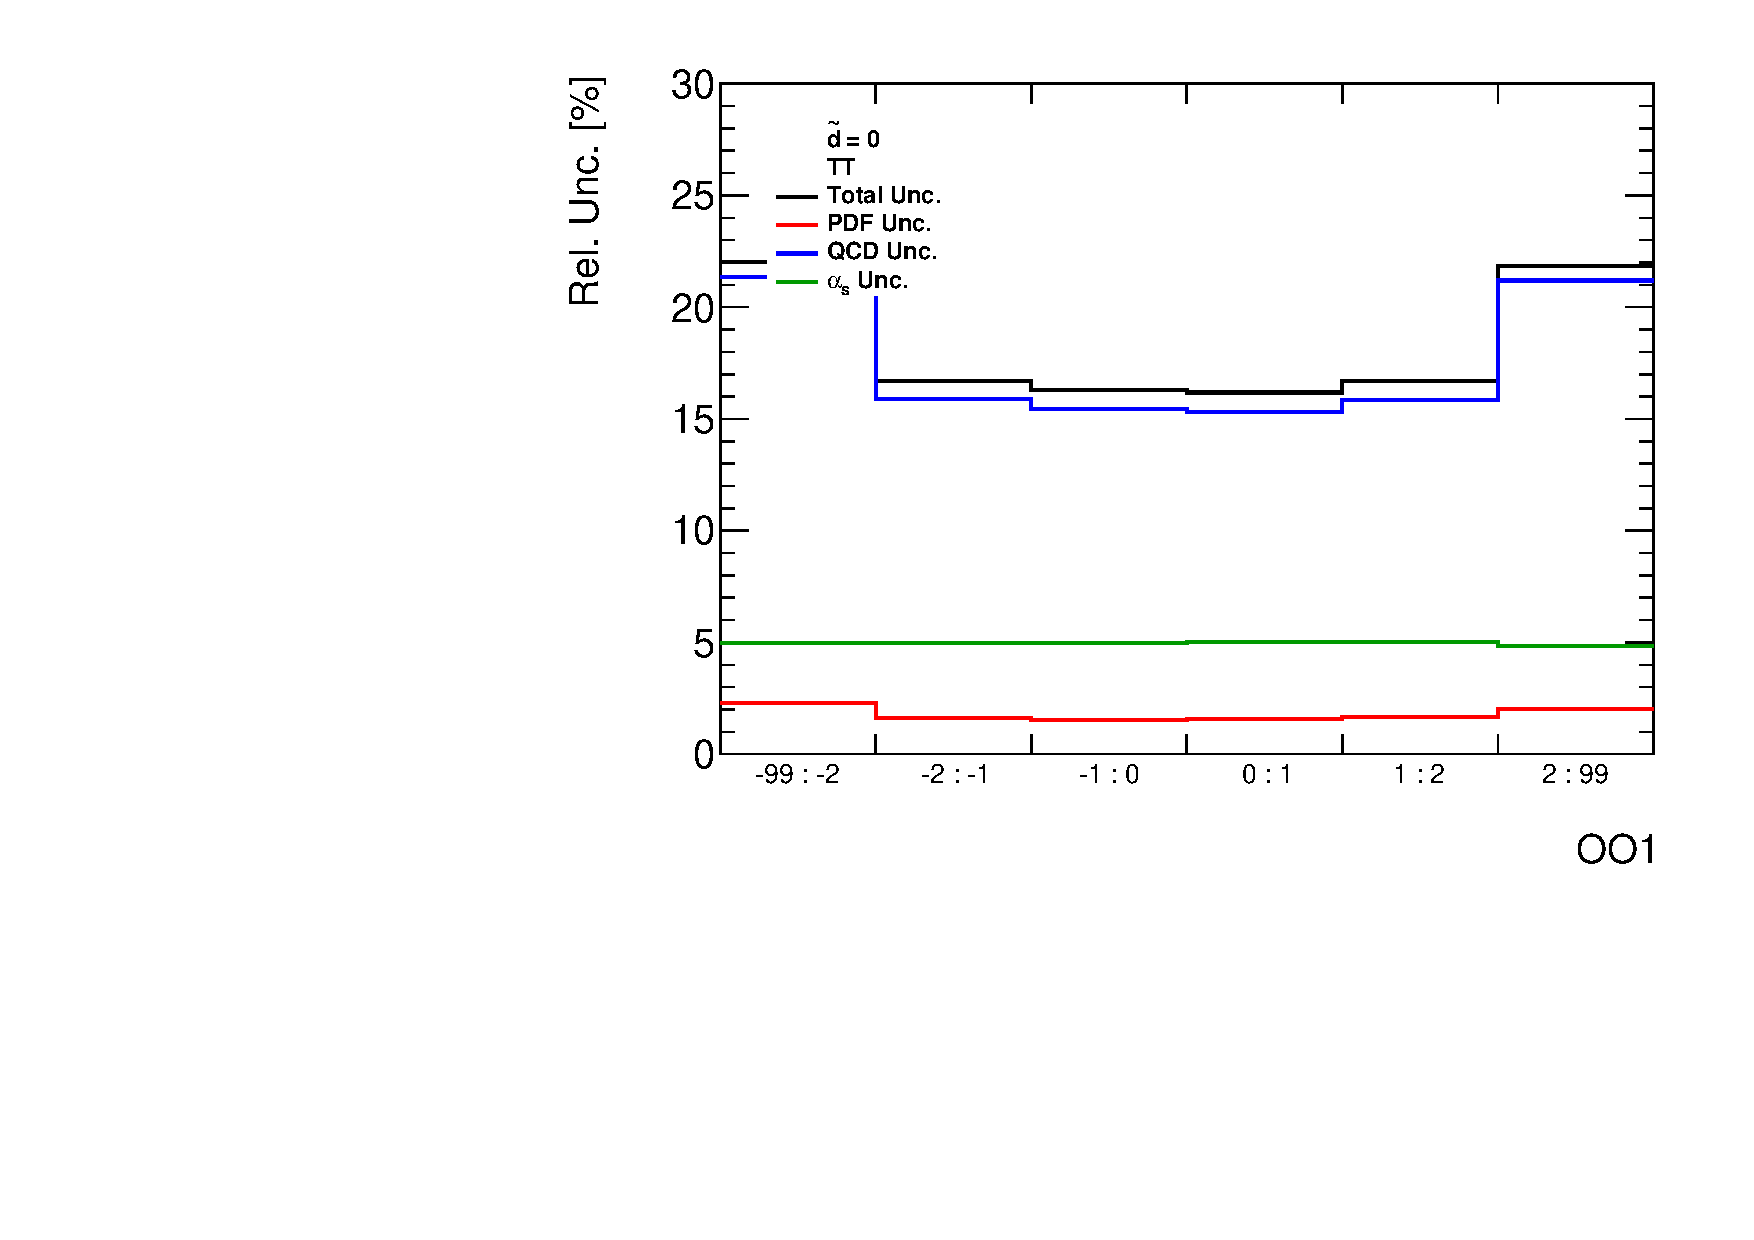
\includegraphics[width= 0.23\textwidth]{figure/TheorySyst/ggF_theoryUnc_TT_d_0.pdf} }
  \subfloat[TL ]{ 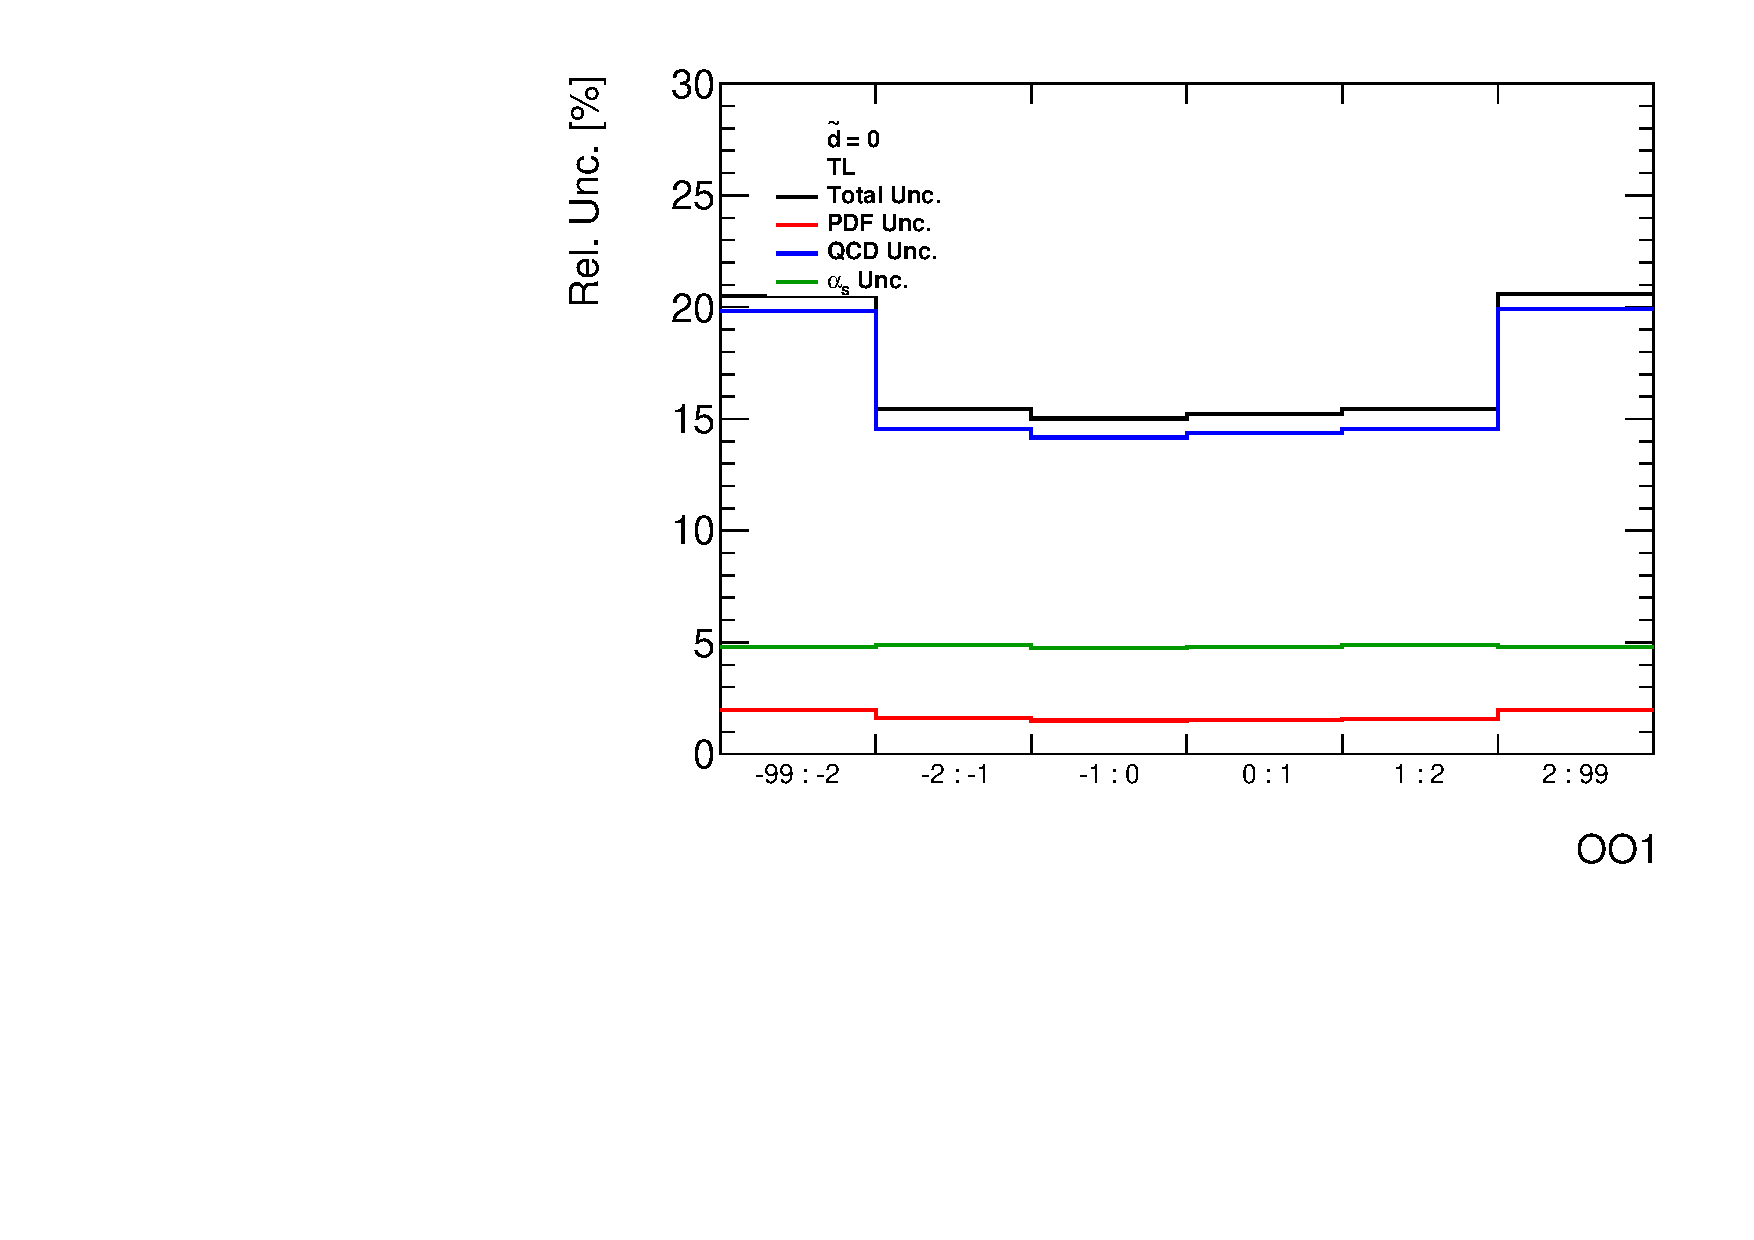
\includegraphics[width= 0.23\textwidth]{figure/TheorySyst/ggF_theoryUnc_TL_d_0.pdf} }
  \subfloat[LT ]{ 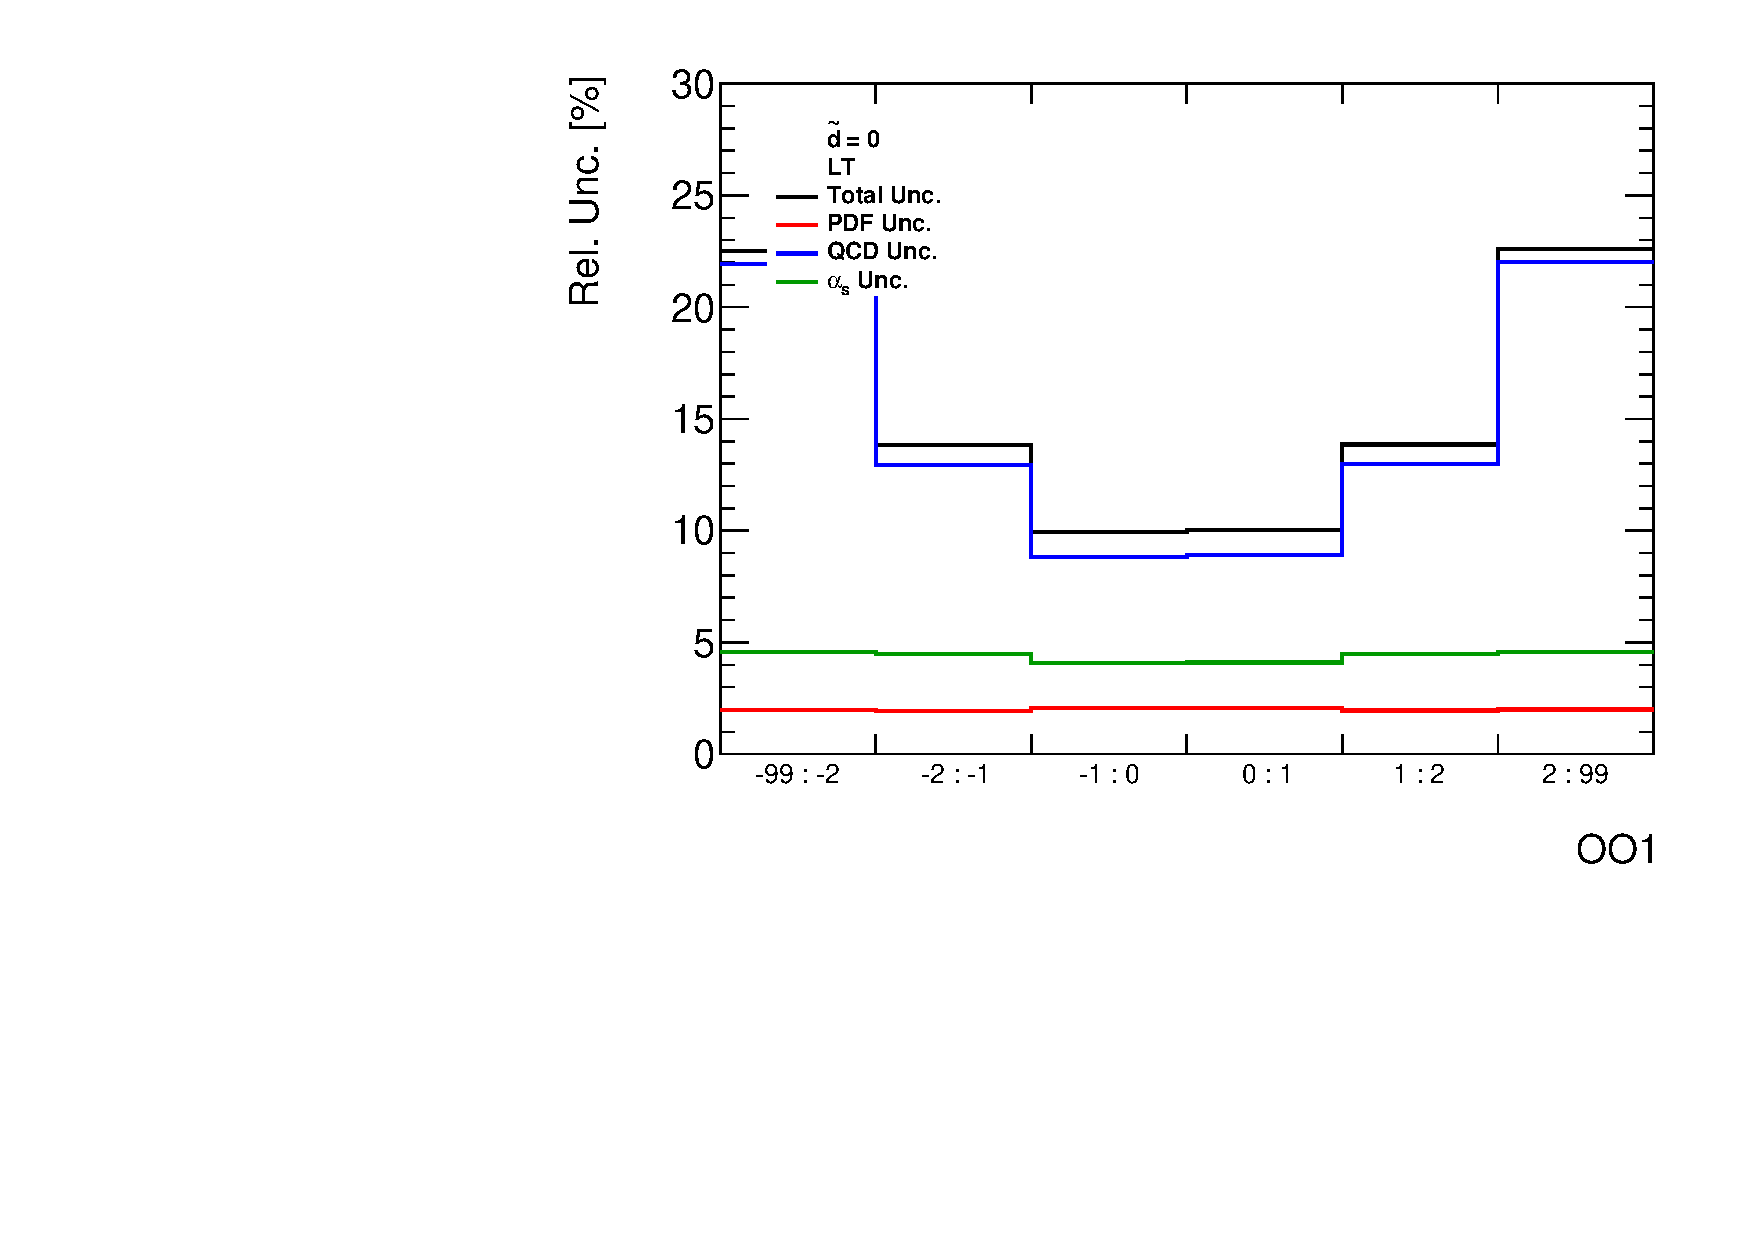
\includegraphics[width= 0.23\textwidth]{figure/TheorySyst/ggF_theoryUnc_LT_d_0.pdf} } 
  \subfloat[LL ]{ 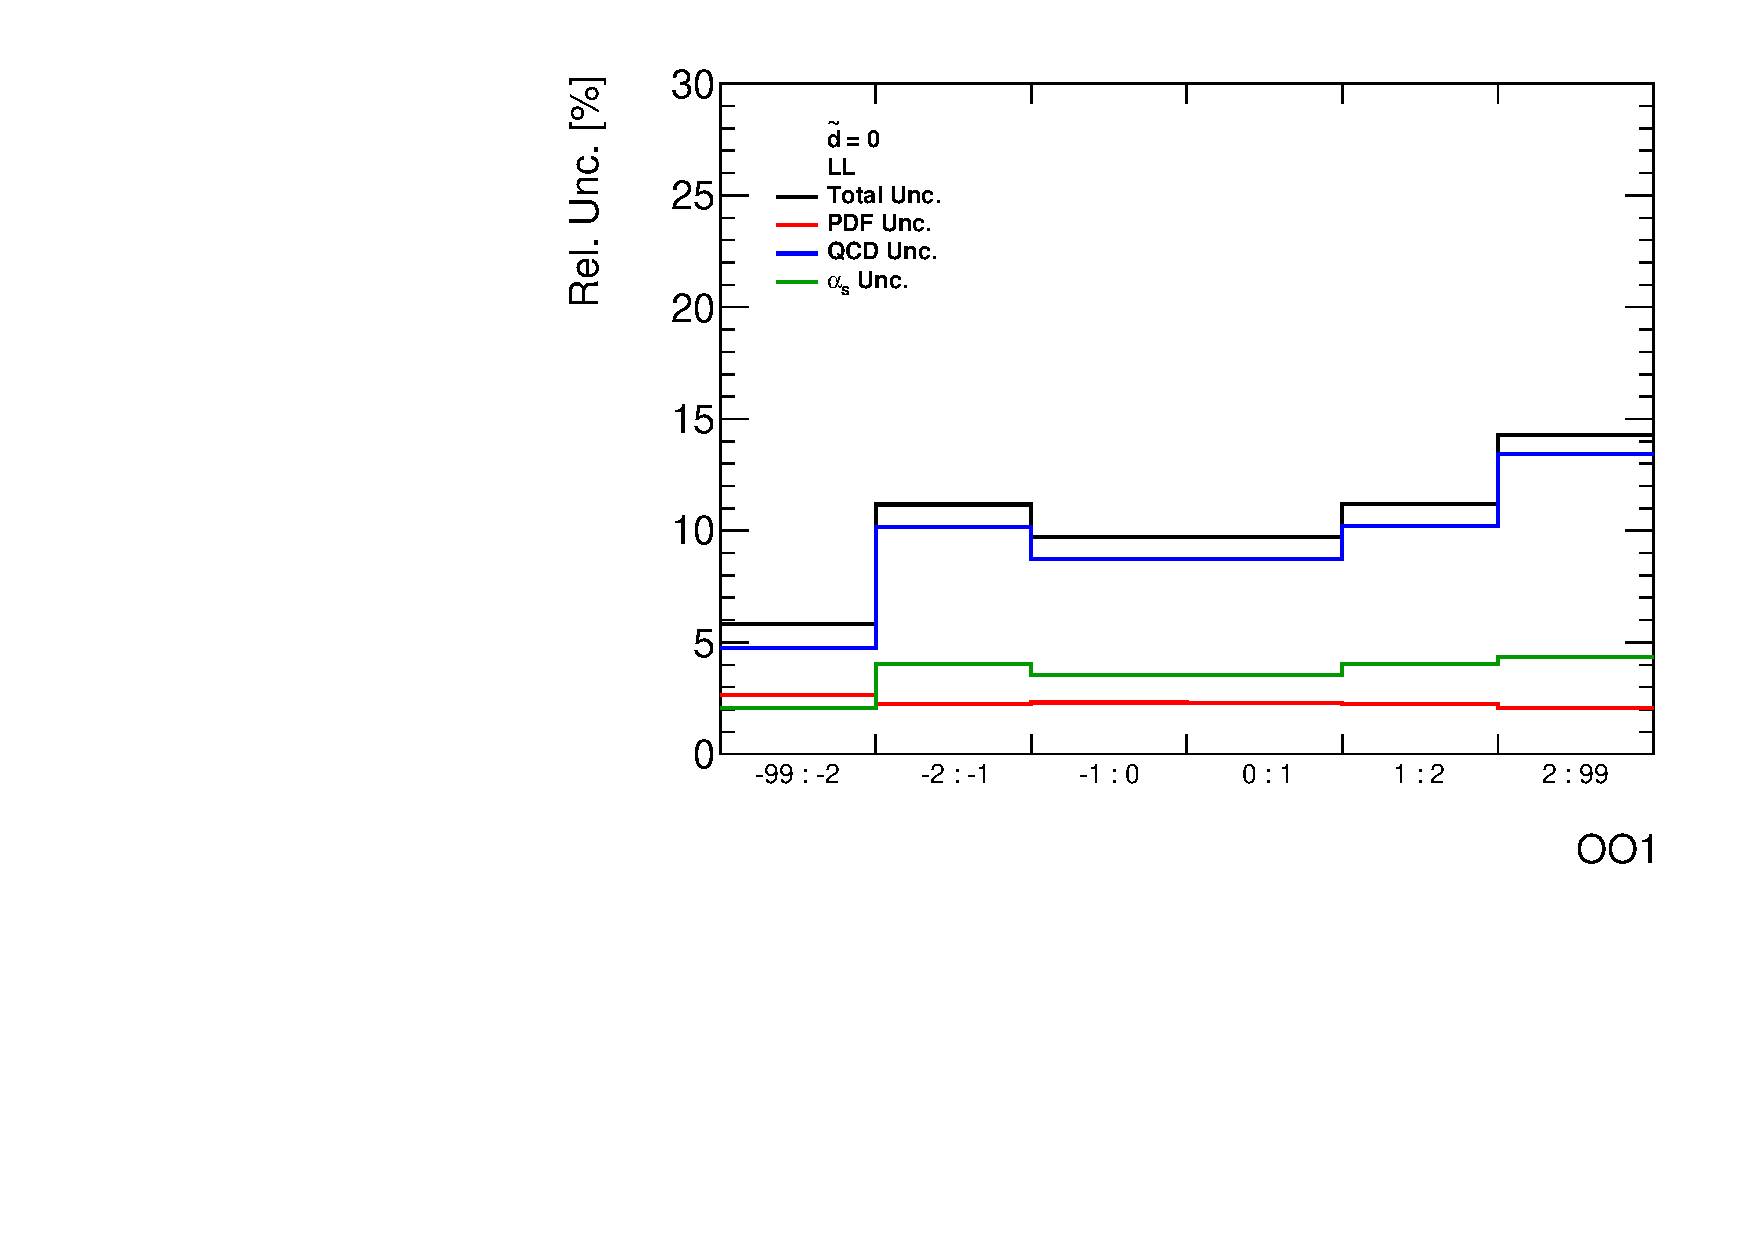
\includegraphics[width= 0.23\textwidth]{figure/TheorySyst/ggF_theoryUnc_LL_d_0.pdf} } 
  \caption{Theory uncertainty in different OO bins for ggF process}
  \label{fig:theoryUnc_ggF}
\end{figure}

\begin{figure}[htbp]
\centering
  \subfloat[TT ]{ 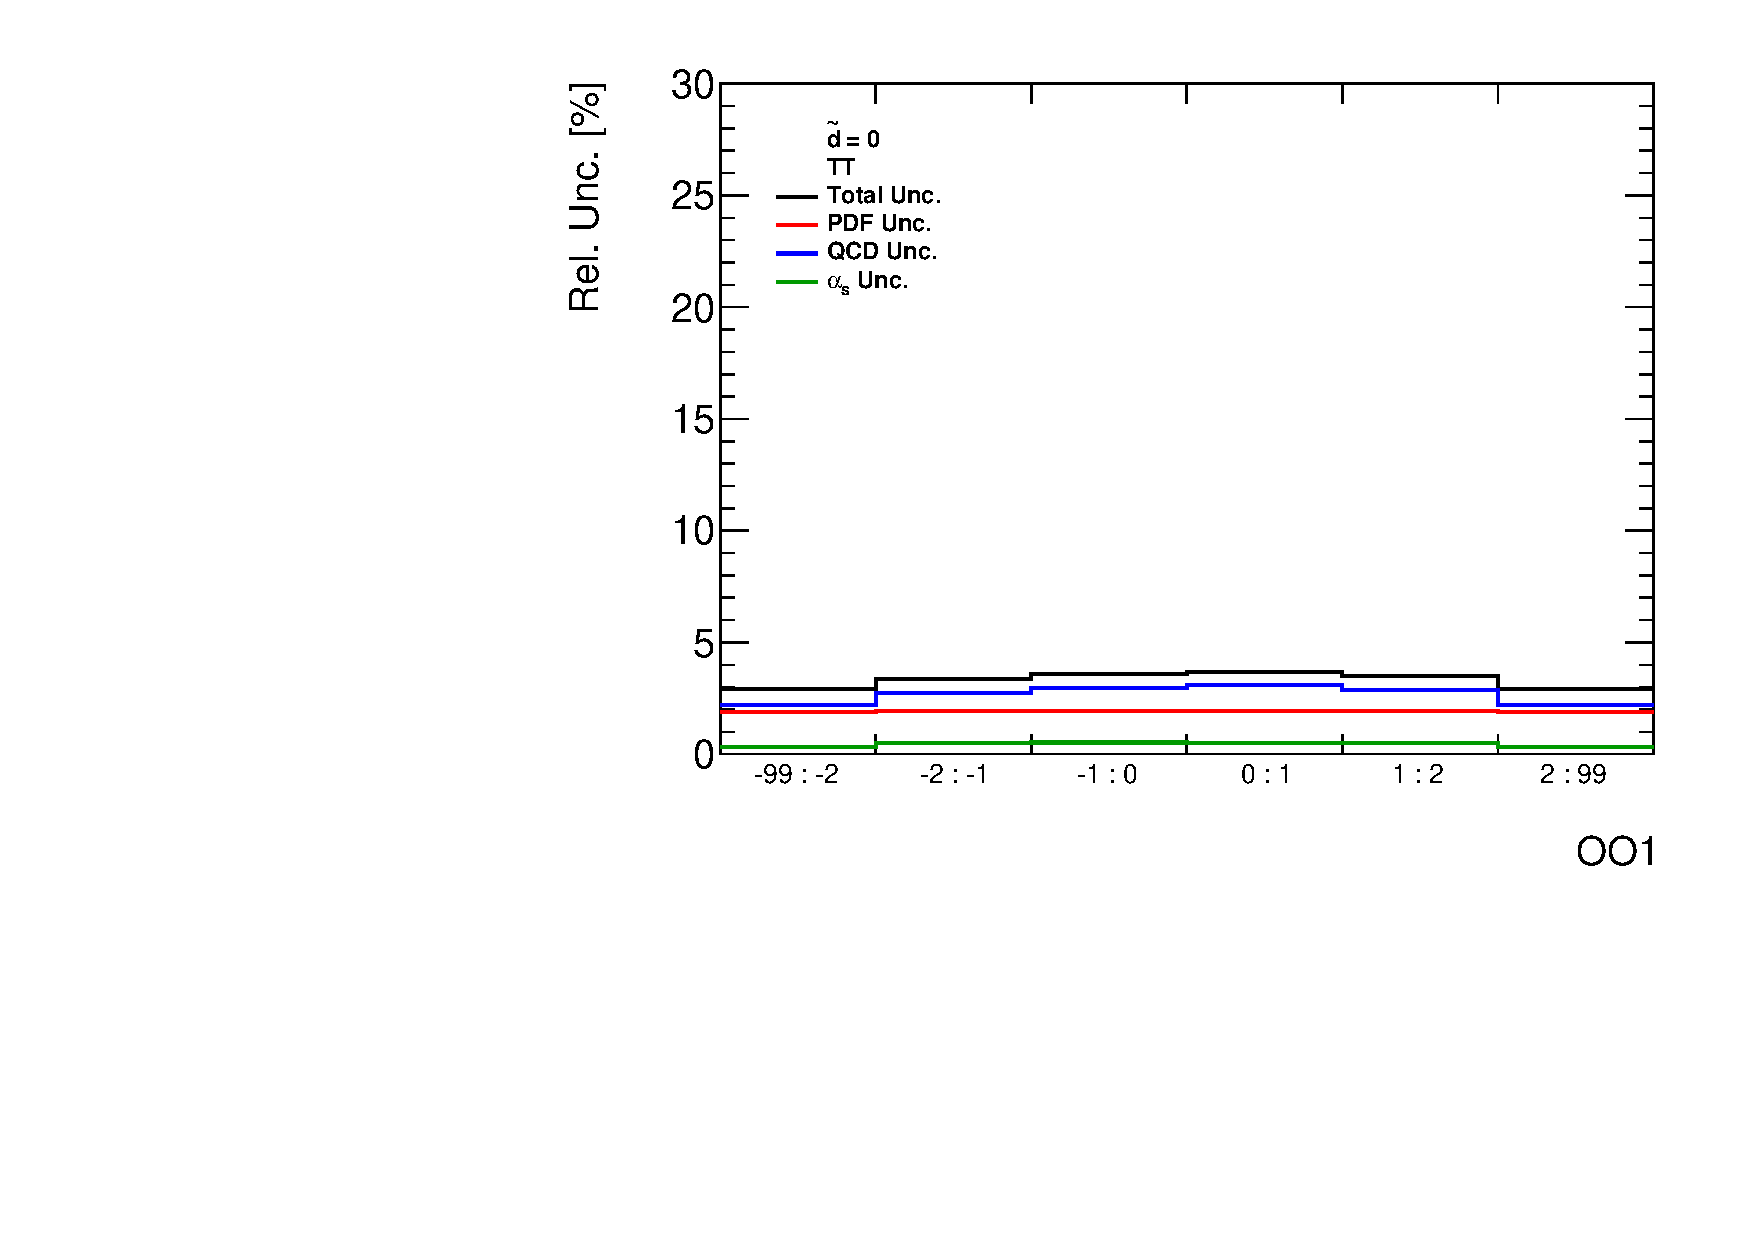
\includegraphics[width= 0.23\textwidth]{figure/TheorySyst/VBF_theoryUnc_TT_d_0.pdf} }
  \subfloat[TL ]{ 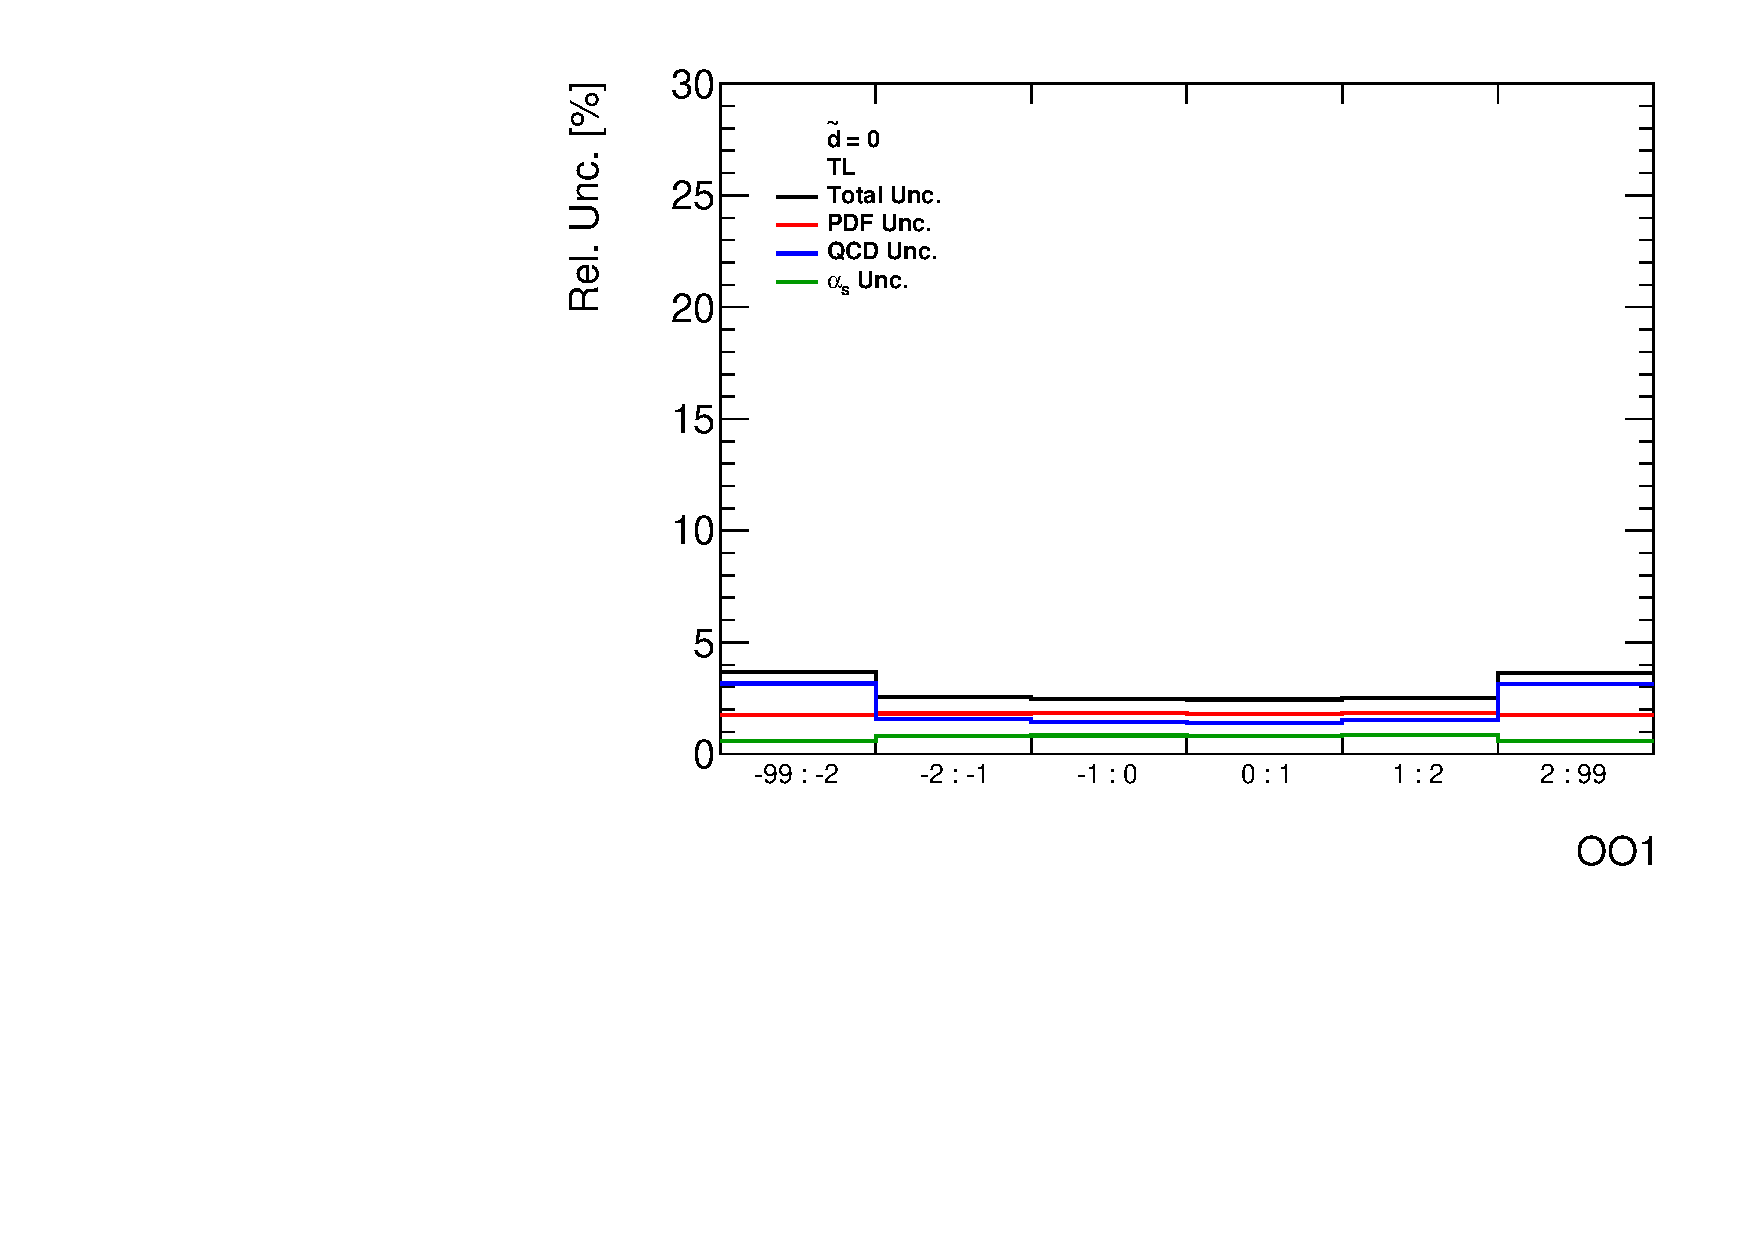
\includegraphics[width= 0.23\textwidth]{figure/TheorySyst/VBF_theoryUnc_TL_d_0.pdf} }
  \subfloat[LT ]{ 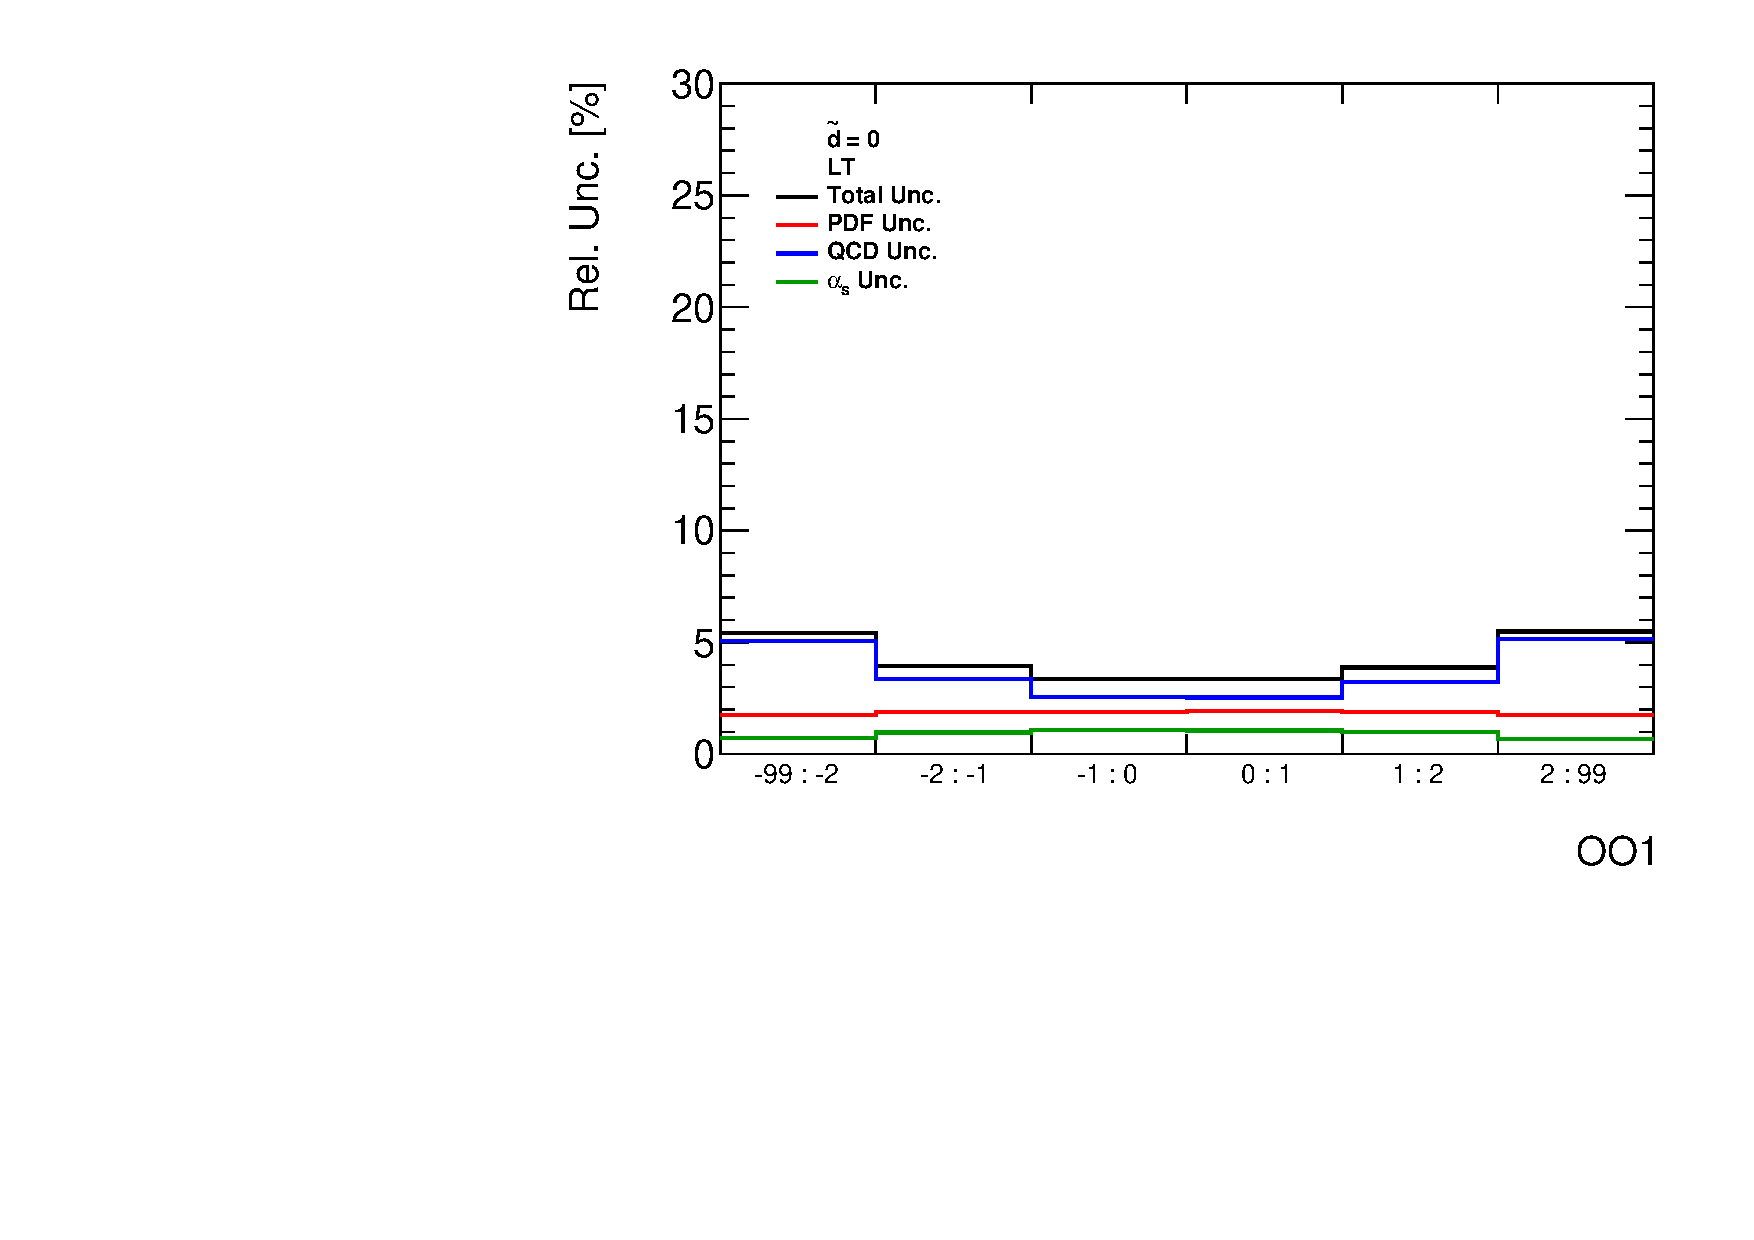
\includegraphics[width= 0.23\textwidth]{figure/TheorySyst/VBF_theoryUnc_LT_d_0.pdf} }
  \subfloat[LL ]{ 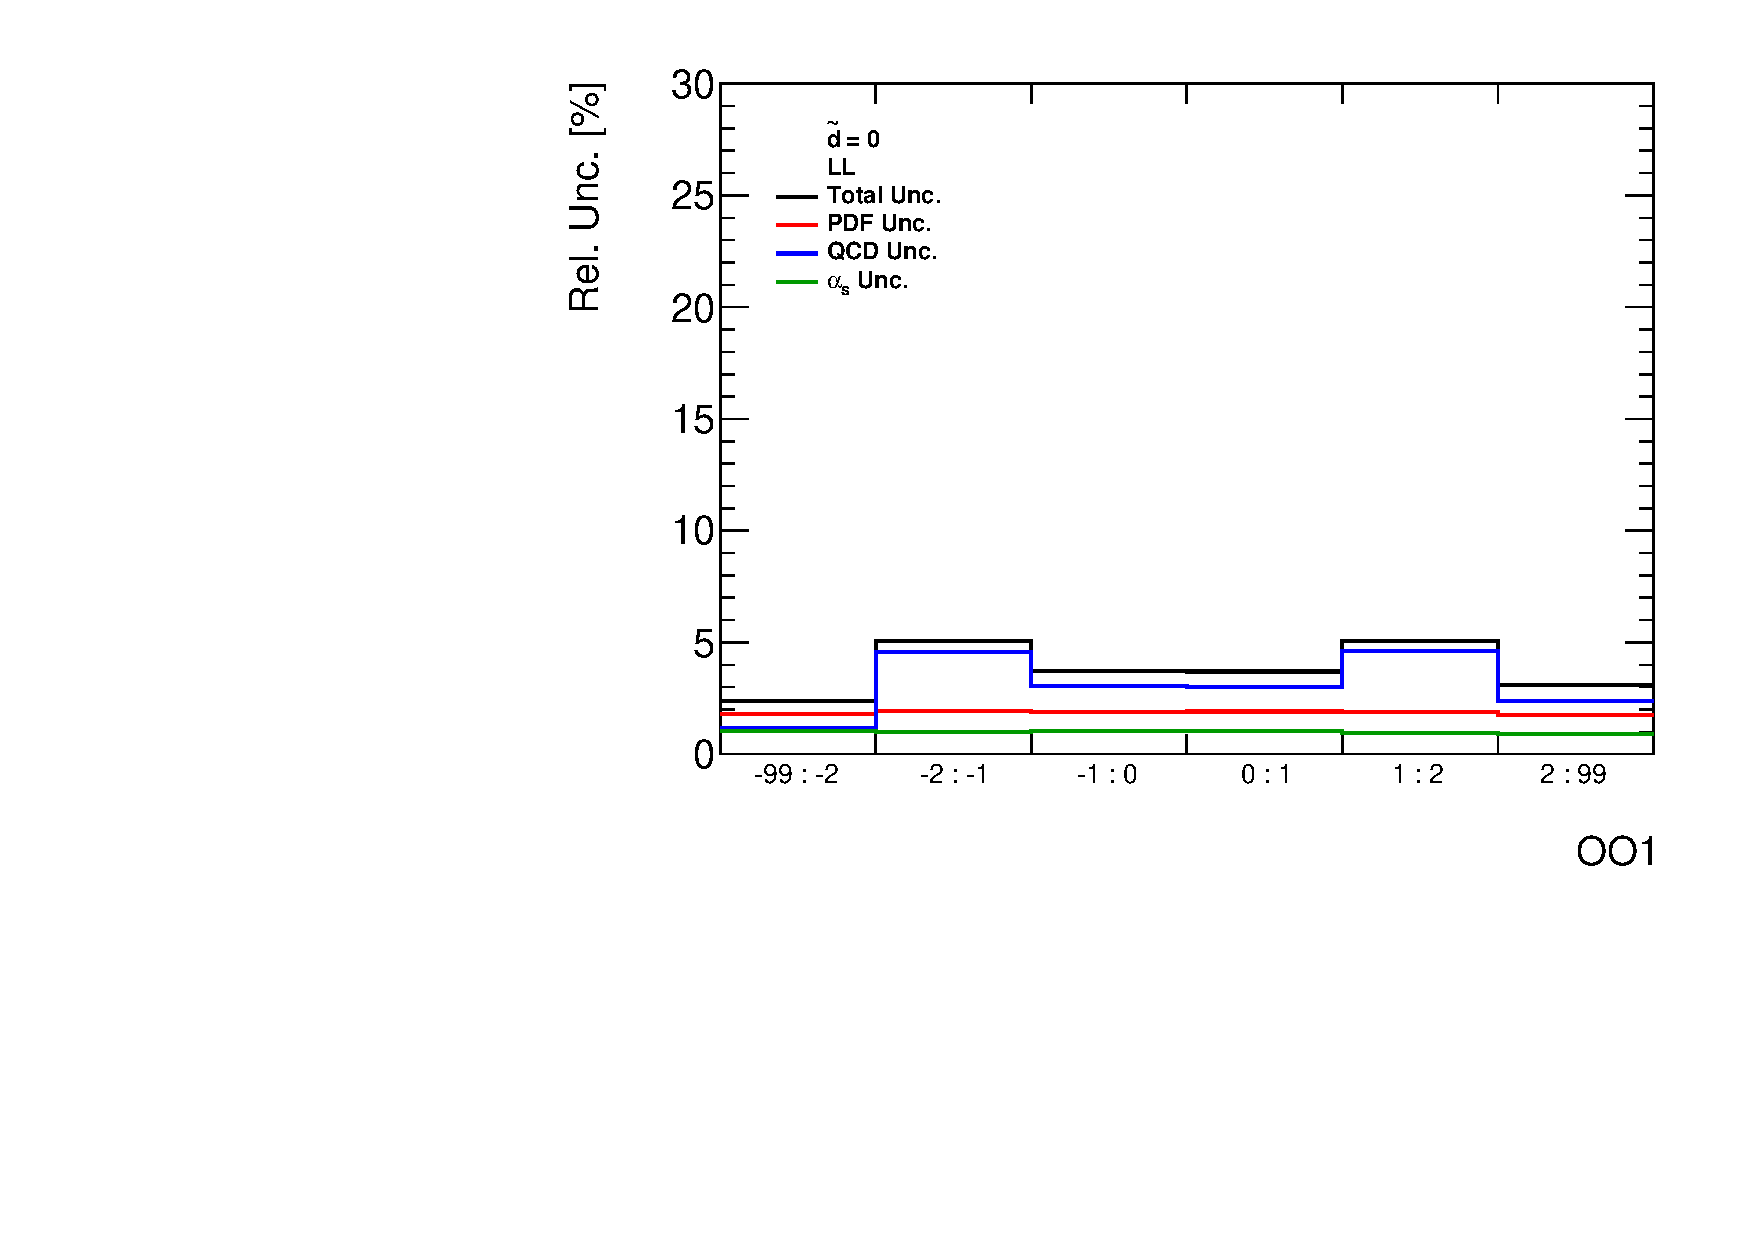
\includegraphics[width= 0.23\textwidth]{figure/TheorySyst/VBF_theoryUnc_LL_d_0.pdf} }
  \caption{Theory uncertainty in different OO bins for VBF process}
  \label{fig:theoryUnc_VBF}
\end{figure}




\subsection{Uncertainties from signal and background modeling}
\label{ssec:modeluncert}

\paragraph{} The Higgs peak described by double-side crystal ball function can be influence by several experimental effects. 
Photon energy scale uncertainties shift the position of signal peak by between $\pm0.2\%$ and $\pm0.4\%$, while the photon resolution uncertainties change the width of signal peak by between $\pm 6\%$ and $\pm 15\%$, following Ref ~\cite{ref:phscaleres}. 
Uncertainty due to knowledge of Higgs boson mass of 0.24GeV ~\cite{ref:mHerror} would also affect the signal peak position. 
These sources are considered independently into systematic uncertainties. 
\# \textcolor{red}{NUMBER NEED CHECK}
\todo{either add tables with full numbers here or in the signal section}
\paragraph{} The uncertainty due to the background choice is taken to be the spurious signal yield discussed in \Sect{\ref{ssec:spurious_signal}}, and assumed to be uncorrelated in each bins. 


\subsection{Experimental systematic uncertainties affecting the expected signal yields}
\label{ssec:expuncert}
\todo{too concise, please detail and split jet, photons sources and write one line how these variations are estimated, add OO plots showing the sys. variations (i have those plots)}
\paragraph{} With data taken during 2015-2018, the uncertainty from integrate luminosity is 2.0\%. Other sources of experimental uncertainty affecting the expected signal yields include: the efficiency of diphoton trigger, the photon identification and isolation efficiencies, the photon energy scale and resolution, the modelling of pile-up in the simulation, the jet energy scale and resolution, the efficiency of the jet vertex tagger. Among them the dominant one is jet flavor composition \texttt{ATLAS\_JET\_Flavor\_Composition} which contributes 5.5\%. \\

The considered systematic uncertainty terms are shown in Figure ~\ref{fig:syst_ranking}. 

\todo{the ranking plot doesn't belong in this section, should be in the next}
\begin{figure}[h]
  \centering
  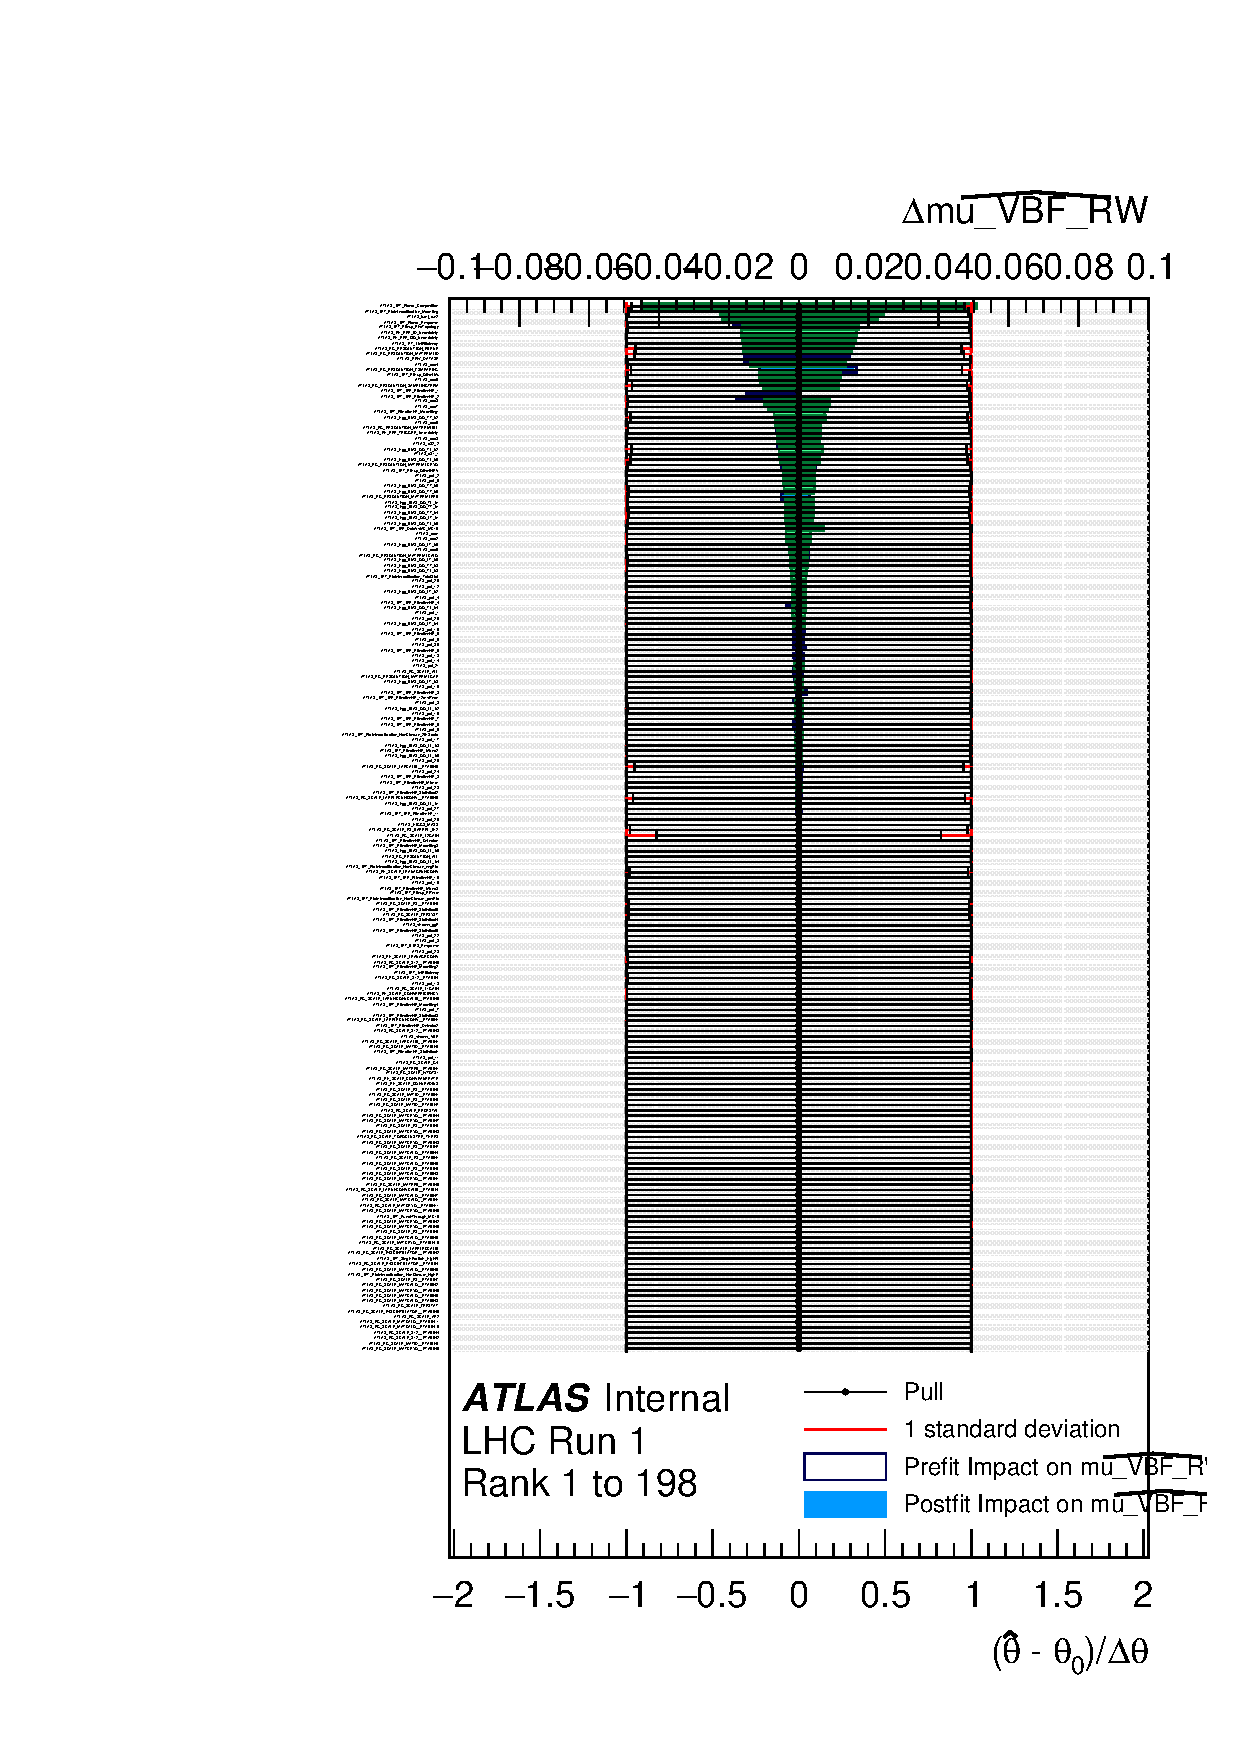
\includegraphics[width=.9\textwidth]{figure/ranking.pdf}
  \caption{Ranking plot for all systematic uncertainty terms. }
  \label{fig:syst_ranking}
\end{figure}


